\documentclass[../main.tex]{subfiles}
\begin{document}
\chapter{Requirements Engineering}
Per essere sicuri che una soluzione software risolva correttamente un problema del mondo reale dobbiamo prima comprenderlo completamente e definire: 
\begin{itemize}
	\item Quale problema sia da risolvere
	\item Il contesto da cui il problema parte
\end{itemize}
Definiamo come \textbf{mondo} la parte problematica del mondo reale, composto da componenti umani e componenti fisici.
Chiamiamo invece \textbf{macchina} (o sistema) ciò che deve essere installato per risolvere il problema, cioè software o soluzione hardware-software.
Il requirements engineering (RE) riguarda gli effetti della macchina sul mondo reale, le assunzioni e proprietà rilevanti del mondo.
\\ 
Il \textbf{system as-is} è il sistema allo stato attuale, precedente l'installazione della macchina.
Il \textbf{system to-be} è il sistema futuro, come sarà una volta installata la macchina.
\\
In una definizione preliminare di RE possiamo dire che è un insieme di attività volto a esplorare, valutare, documentare, consolidare, ripassare e adattare gli obiettivi, capacità, qualità, requisiti e assunzioni di un sistema software-intensive.
È basato sui problemi che sorgono nel sistema as-is e le opportunità portate dalle nuove tecnologie.
Le difficoltà principali del RE sono:
\begin{itemize}
	\item Scope ampio: diverse versioni del software (as-is, to-be, to-be-next) e ambienti ibridi (organizzazioni, leggi, politiche, device)
	\item Considerazioni multiple: funzionali, di qualità, di sviluppo.
	\item Livelli di astrazione
	\item Stakeholder multipli: con background diversi, interessi diversi e punti di vista contrastanti.
	\item Task intersecate durante il processo iterativo di elicitazione, valutazione, specifica e consolidazione.
\end{itemize}
Tre domande fondamentali che dobbiamo porci sono: perché installare un nuovo sistema? Quali servizi? Chi è responsabile per cosa?
\begin{itemize}
	\item \textbf{Perché?} Identificare, analizzare, rifinire gli obiettivi del sistema to-be per risolvere problematiche rilevate nel sistema as-is, allinearsi con gli obiettivi business e sfruttare nuove tecnologie.
	\\
	Le difficoltà principali sono:
	\begin{itemize}
		\item Acquisire conoscenze del dominio
		\item Valutare le varie alternative
		\item Identificare e risolvere conflitti tra obiettivi
	\end{itemize}
	\item \textbf{Cosa?} Identificare, definire i servizi funzionali del sistema to-be
	\begin{itemize}
		\item Soddisfare gli obiettivi identificati 
		\item In concomitanza con i requisiti di qualità: prestazioni, sicurezza\dots
		\item Basarsi su assunzioni realistiche dell'ambiente.
	\end{itemize}
	Le difficoltà principali sono:
	\begin{itemize}
		\item Identificare le feature corrette.
		\item Specificarle in maniera precisa in maniera che tutti possano capire.
		\item Assicurare la tracciabilità tra obiettivi.
	\end{itemize}
	\item \textbf{Chi?} Assegnare le responsabilità per gli obiettivi, servizi requisiti tra i componenti del sistema to-be.
	\begin{itemize}
		\item Basandosi sulle capacità e obiettivi del sistema.
		\item Definire il limite tra software e ambiente.
	\end{itemize}
	Le difficoltà principali sono:
	\begin{itemize}
		\item Valutare soluzioni alternative per decidere il giusto livello di automazione.
	\end{itemize}
\end{itemize}
\section{Tipi di requisiti}
Il modo in cui i requisiti vengono espressi possono essere divisi in \textbf{descrittivi} (modo indicativo) e \textbf{prescrittivo} (modo ottativo).
\\
\begin{tikzpicture}[
    node distance=2cm and 2.8cm,
    box/.style={
        draw,
        thick,
        rounded corners,
        fill=blue!10,
        align=center,
        minimum width=3.8cm,
        minimum height=1cm,
        font=\bfseries
    },
    arrowblue/.style={-Latex, thick, blue!70!black},
    arrowblack/.style={-Latex, thick, black}
]

% Nodes
\node[box] (env) {Environment};
\node[box, above=of env] (input) {Input Devices\\\normalsize(e.g.\ sensors)};
\node[box, above right=of env] (soft) {SoftwareToBe};
\node[box, right=of env] (output) {Output Devices\\\normalsize(e.g.\ actuators)};

% Arrows with side labels
\draw[arrowblack] (env) -- (input)
    node[midway, above left=2pt and 2pt] {\small M: monitored variables};

\draw[arrowblack] (input) -- (soft)
    node[midway, above =2pt and 2pt] {\small I:input data};

\draw[arrowblack] (soft) -- (output)
    node[midway, below right=2pt and 2pt] {\small O: output signals};

\draw[arrowblack] (output) -- (env)
    node[midway, below =2pt and 2pt] {\small C: controlled vars};

\end{tikzpicture}


\subsection{Requisiti di sistema}
Sistemi prescrittivi che si riferiscono a fenomeni dell'ambiente (non necessariamente condivisi).
Vengono soddisfatti dal sistema to-be, possibilmente integrato con altri componenti del sistema. Devono essere comprensibili da tutti gli stakeholder.
$SysReq\subseteq M\times C$ relazione tra ambiente monitorato e variabili controllate.
\subsection{Requisiti software}
Affermazioni prescrittive che si riferiscono a fenomeni condivisi tra ambiente e software. Vengono soddisfatti unicamente dal software, formulati nel vocabolario degli sviluppatori.
$SofReq\subseteq I\times O$ relazione tra input e output del software.
\subsection{Proprietà di dominio}
Affermazioni descrittive riguardanti i fenomeni del mondo (rimangono veri a prescindere del sistema to-be).
$Dom\subseteq M\times C$ leggi che non possono essere violate.
\subsection{Assunzioni}
Affermazioni che l'ambiente del software-to-be deve soddisfare. Formulate in termini di fenomeni di ambiente. Generalmente prescrittive (e.g. sensori e attuatori).
$Asm\subseteq M\times C \cup M\times I \cup C \times O$
\subsection{Definizioni}
Affermazioni che forniscono un preciso significato ai concetti di sistemi e termini ausiliari.
Non hanno valore di verità, non ha senso contestarle.
$sofReq=Map(SysReq, Asm, Dom)$
\\ \\
I requisiti si dividono ulteriormente in:
\begin{itemize}
	\item \textbf{Funzionali}: descrivono quali servizi il sistema deve fornire.
	\item \textbf{Non funzionali}: descrivono come il sistema deve essere (e.g. prestazioni, usabilità, affidabilità\dots).
\end{itemize}
\section{Qualità del software}
\begin{itemize}
    \item Completezza di obiettivi, requisiti e assunzioni
    \item Coerenza degli elementi del documento dei requisiti (RD)
    \item Adeguatezza di requisiti, assunzioni e proprietà del dominio
    \item Non ambiguità degli elementi del documento dei requisiti
    \item Misurabilità di requisiti e assunzioni
    \item Pertinenza di requisiti e assunzioni
    \item Fattibilità dei requisiti
    \item Comprensibilità degli elementi del documento dei requisiti
    \item Buona strutturazione del documento dei requisiti
    \item Modificabilità degli elementi del documento dei requisiti
    \item Tracciabilità degli elementi del documento dei requisiti
\end{itemize}
Errori nei documenti dei requisiti:
\begin{itemize}
    \item \textbf{Omissione:} caratteristica del mondo del problema non indicata in alcun elemento del documento dei requisiti (RD).\\
    \emph{Esempio:} nessun requisito riguardante lo stato delle porte del treno in caso di arresto di emergenza.
    
    \item \textbf{Contraddizione:} elementi del RD che descrivono una caratteristica del mondo del problema in modo incompatibile.\\
    \emph{Esempio:} ``Le porte devono essere sempre tenute chiuse tra le piattaforme'' e ``Le porte devono essere aperte in caso di arresto di emergenza.''
    
    \item \textbf{Inadeguatezza:} elemento del RD che non descrive in modo adeguato una caratteristica del mondo del problema.\\
    \emph{Esempio:} ``Se un libro non è stato restituito, il prestatore negligente deve essere avvisato che deve pagare una multa.''
    
    \item \textbf{Ambiguità:} elemento del RD che permette di interpretare una caratteristica del mondo del problema in modi diversi.\\
    \emph{Esempio:} ``Solo le persone che hanno partecipato ad almeno il 75\% delle riunioni possono essere premiate alla fine dell’anno.''
    
    \item \textbf{Non misurabilità:} elemento del RD che descrive una caratteristica del mondo del problema in modo tale da impedire il confronto tra opzioni o la verifica delle soluzioni.
\end{itemize}
Difetti nei documenti dei requisiti:
\begin{itemize}
    \item \textbf{Rumore (Noise):} elemento del RD che non fornisce alcuna informazione su caratteristiche del mondo del problema.\\
    \emph{Variante: ridondanza incontrollata.}\\
    \emph{Esempio:} ``Devono essere affissi cartelli di divieto di fumo sui finestrini del treno.''
    
    \item \textbf{Sovraspecificazione (Overspecification):} elemento del RD che descrive una caratteristica non presente nel mondo del problema, ma nella soluzione della macchina.\\
    \emph{Esempio:} ``Il metodo setAlarm deve essere invocato al ricevimento di un messaggio Alarm.''
    
    \item \textbf{Non fattibilità (Unfeasibility):} elemento del RD non implementabile entro i vincoli di budget o tempi.\\
    \emph{Esempio:} ``I pannelli a bordo del treno devono visualizzare tutti i voli in ritardo alla prossima fermata.''
    
    \item \textbf{Inintelleggibilità (Unintelligibility):} elemento del RD incomprensibile per chi deve utilizzarlo.\\
    \emph{Esempio:} ``Negli Stati Uniti, la nozione di NWO è diventata popolare dopo gli attacchi terroristici al WTC. Tuttavia, i funzionari della NATO e dell’OMC raramente fanno riferimento a un NWO nelle procedure relative al GATT, e si può dire che MVTO, la clausola MFN e gli SRO abbiano poco a che fare con un NOW.'' (da un comunicato stampa)
    
    \item \textbf{Scarsa strutturazione (Poor structuring):} elemento del RD non organizzato secondo alcuna regola sensata e visibile di strutturazione.\\
	\emph{Esempio:} ``Interconnessione dei controllo di accelerazione e problemi al tracking del treno``
    \item \textbf{Riferimento anticipato (Forward reference):} elemento del RD che utilizza caratteristiche del mondo del problema non ancora definite.\\
    \emph{Esempio:} uso multiplo del concetto di distanza di arresto nel caso peggiore prima che la sua definizione appaia alcune pagine dopo nel RD.
    
    \item \textbf{Rimpianto (Remorse):} elemento del RD che definisce una caratteristica del mondo del problema in modo tardivo o incidentale.\\
    \emph{Esempio:} dopo molteplici utilizzi del concetto non definito di distanza di arresto nel caso peggiore, l’ultimo uso è seguito direttamente da una definizione incidentale tra parentesi.
    
    \item \textbf{Scarsa modificabilità (Poor modifiability):} elementi del RD i cui cambiamenti devono essere propagati in tutto il documento.\\
    \emph{Esempio:} uso di valori numerici fissi per quantità soggette a variazioni.
    
    \item \textbf{Opacità (Opacity):} elemento del RD il cui razionale, autore o dipendenze sono invisibili.\\
    \emph{Esempio:} ``La velocità comandata del treno deve essere sempre almeno 7 mph superiore alla velocità fisica'' senza alcuna spiegazione del razionale di questa scelta.
\end{itemize}
\section{Processo di RE}
\begin{figure}[h]
    \centering
    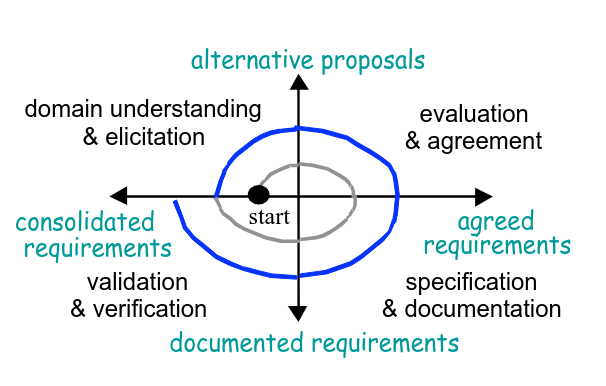
\includegraphics[width=0.7\textwidth]{pictures/RE.png}
\end{figure} \noindent
Per comprendere il dominio bisogna studiare il sistema as-is, identificare gli stakeholders, così da generare delle prime proposte di prototipi e il glossario dei termini.
\subsection{Elicitazione dei requisiti}
L'\textbf{elicitazione} dei requisiti esplora i problemi del mondo facendo ulteriori analisi del problema del sistema as-is, individuandone i sintomi, cause e conseguenze.
Vengono identificati:
\begin{itemize}
	\item Opportunità tecnologiche
	\item Obiettivi di miglioramento
	\item Requisiti tecnico-organizzativi del sistema to-be
	\item Soluzioni alternative per soddisfare gli obiettivi e assegnare le responsabilità
	\item Scenari ipotetici di interazione software-ambiente
	\item Requisiti software, assunzioni sull'ambiente
\end{itemize}
\subsection{Evaluazione e negoziazione dei requisiti}
Presa di decisioni basate sulla negoziazione. 
\begin{itemize}
	\item Identificazione e risoluzione di conflitti 
	\item Identificazione e risoluzione dei rischi del sistema proposto
	\item Confronto delle alternative tra obiettivi e rischi, selezione della soluzione preferita
	\item Priorità dei requisiti, per risolvere conflitti, considerare costi e supportare lo sviluppo incrementale.
\end{itemize}
Vengono prodotti le sezioni finali della proposta di prototipo che documentano gli obbiettivi concordati, i requisiti, le assunzioni e i ragionamenti che hanno portato ad essi.
\subsection{Specifiche e documentazione}
Definizione precisa di tutte le feature del sistema.
Obiettivi, proprietà di dominio rilevanti, requisiti, assunzioni, responsabilità.
Organizzare questi in una struttura coerente. Documentare in una forma comprensibile a tutti gli interessati. Viene prodotto il Requirements Document (RD).
\subsection{Consolidazione dei requisiti}
Attività per assicurare la qualità del RD. Vengono analizzate l'adeguatezza, la completezza, la mancanza di inconsistenze, vengono poi sistemati gli errori e i difetti. Viene prodotto un RD consolidato.
\section{Analisi di dominio ed elicitazione dei requisiti}
Il processo prevede:
\begin{itemize}
	\item Identificare gli stakeholder e interagire con loro.
	\item Applicare tecniche di elicitazione \textit{artefact-driven}.
	\begin{itemize}
		\item Studio di background
		\item Raccoglimento dati e questionari
		\item Griglie di repertorio, card sorting per acquisizione di concetti.
		\item Scenari, storyboard per esplorare i problemi del mondo.
		\item Prototipi, mock-up per feedback rapido.
	\end{itemize}
	\item Tecniche di elicitazione \textit{stakeholder-driven}.
	\begin{itemize}
		\item Interviste.
		\item Osservazioni e studi etnografici.
		\item Sessioni di gruppo.
	\end{itemize}
\end{itemize}
Per comprendere i problemi del mondo è necessario selezionare stakeholder rappresentativi, gli aspetti rilevanti sono;
\begin{itemize}
	\item Posizione nell'organizzazione.
	\item Ruolo nelle decisioni sul sistema to-be.
	\item Livello di conoscenza del dominio.
	\item Esposizione ai problemi percepiti.
	\item Influenza sull'accettazione del sistema.
	\item Obiettivi personali e conflitti di interessi.
\end{itemize}
\begin{figure}[h]
	\centering
	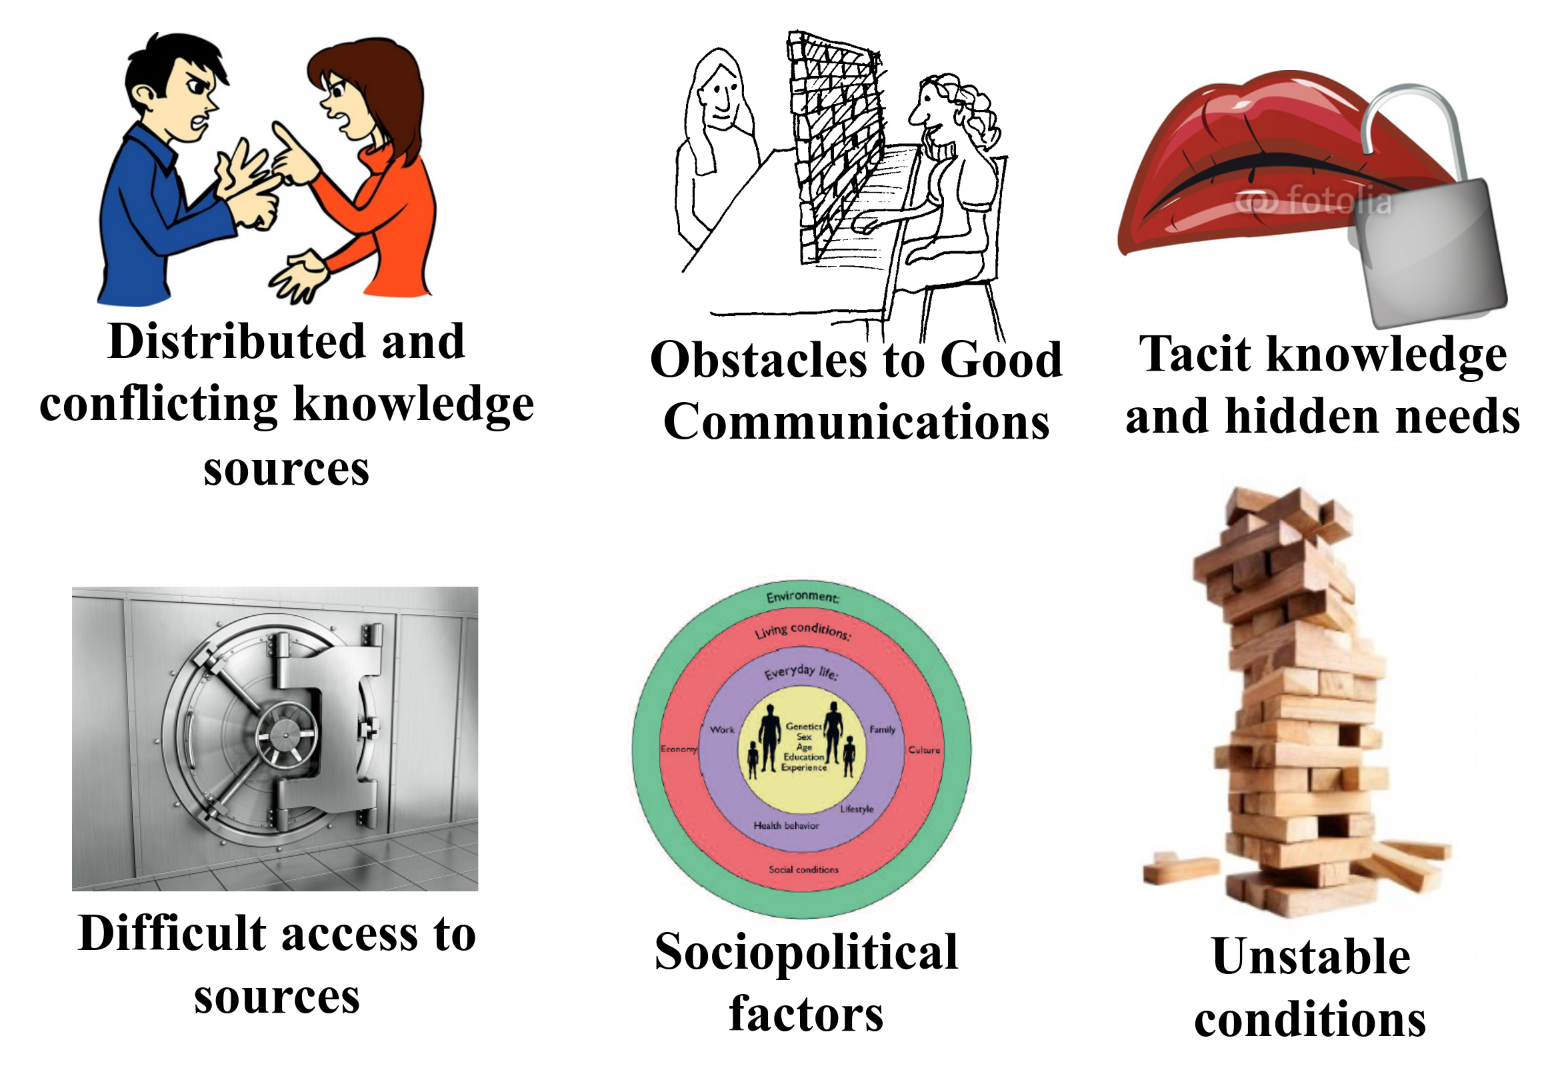
\includegraphics[width=0.7\textwidth]{pictures/ostacoliAcquisizione.png}
	\caption{Ostacoli nell'acquisizione dei requisiti}
\end{figure}
L'interazione con gli stakeholder richiede skill di comunicazione: utilizzare la giusta terminologia, affrontare i punti chiave, fondare relazioni di fiducia.
Per riformulare le conoscenze è necessario organizzare meeting per presentare la conoscenza del mondo, acquisita da fonti diverse, per integrarle in una forma strutturata.
\section{Tecniche di elicitazione artefact-driven}
Effettuare uno studio di background comprende acquisire, leggere e sintetizzare documenti riguardo:
\begin{itemize}
	\item L'\textbf{organizzazione}: diagrammi di organizzazione, business plan, report finanziari, organizzazione meeting, etc \dots
	\item Il \textbf{dominio}: manuali, questionari, articoli, leggi, report su sistemi simili sullo stesso dominio.
	\item Il \textbf{sistema as-is}: workflow documentati, procedure, regole di business, documenti scambiati, report di difetti/lamentele, richieste di cambiamenti, etc \dots
\end{itemize}
Quali sono i problemi degli studi di background?
\begin{itemize}
	\item \textbf{Contro}
	\begin{itemize}
		\item Molti documenti voluminosi vanno letti.
		\item Le informazioni chiave vanno estratte da molti dettagli irrilevanti.
		\item Sfruttare meta-conoscenze per discriminare informazioni rilevanti da quelle inutili.
	\end{itemize}
	\item \textbf{Pro}
	\begin{itemize}
		\item Produce informazioni basilari utili per interagire con gli stakeholder.
	\end{itemize}
\end{itemize}
\subsection{Questionari}
Somministrare una lista di domande a una selezione di stakeholder, ognuna con una lista di possibili risposte (con allegato un breve contesto se necessario).
È possibile somministrare domande a risposta multipla o domande di peso, ovvero una serie di affermazioni d pesare in maniera:
\begin{itemize}
	\item Qualitativa ("alto","basso",\dots)
	\item Quantitativa (percentuale)
	\item Per esprimere la percepita importanza, preferenza, rischio, etc \dots
\end{itemize}
Sono efficaci per acquisire velocemente informazioni soggettive, in maniera economica e remota per molte persone.
Sono utili per preparare meglio interviste più specifiche.
\\
La preparazione va effettuata con molta attenzione in quanto potrebbero introdurre \textbf{bias} o informazioni non affidabili (a causa di incomprensioni delle domande o delle risposte, risposte non consistenti, etc \dots).
Le linee guida per la stesura dei questionari sono:
\begin{itemize}
	\item Selezionare un campione di persone rappresentative e statisticamente significante. Fornire le ragioni dietro queste scelte.
	\item Controllare la copertura delle domande e delle possibili risposte.
	\item Assicurarsi che le domande, le risposte e le formulazioni siano senza bias e non ambigue.
	\item Aggiungere domande implicitamente ridondanti per rilevare risposte incoerenti.
	\item Far controllare il questionario da un ente terzo.
\end{itemize}
\subsection{Storyboard}
Necessaria per acquisire e validare informazioni da esempi concreti riguardanti il sistema as-is e to-be.
Una story board racconta una storia tramite una sequenza di snapshot (frasi, schizzi, slide, immagini\dots) che descrivono un evento o una serie di eventi. Tipicamente annotati da chi è coinvolto, cosa gli succede, perché ciò accade, cosa succede se (non) accade, etc \dots
Può essere formulato in maniera passiva (la storia viene raccontata agli stakeholder) o in maniera attiva (gli stakeholder contribuiscono).
\subsection{Scenari}
Gli scenari illustrano tipiche sequenze di interazioni tra componenti di sistema per raggiungere obiettivi impliciti. Possono essere utilizzati come specifiche di un test case.
Vengono tendenzialmente illustrati tramite testo o diagrammi. Ne esistono di vari tipi:
\begin{itemize}
	\item \textbf{Positivi:} un comportamento che il sistema dovrebbe coprire.
	\item \textbf{Negativi:} un comportamento che il sistema dovrebbe escludere.
	\item \textbf{Normali:} tutto procede come ci si aspetta.
	\item \textbf{Anormali:} una sequenza di una interazione desiderata nel caso di eccezioni (rimane positiva).
\end{itemize}
Gli scenari presentano sia vantaggi che svantaggi, pur essendo probabilmente il metodo di elicitazione più utile:
\begin{itemize}
	\item \textbf{Pro}
	\begin{itemize}
		\item Esempi concreti e contro esempi.
		\item Appetibili per gli stakeholder.
		\item Utilizzabili come test di accettazione.
	\end{itemize}
	\item \textbf{Contro}
	\begin{itemize}
		\item Inerentemente parziali.
		\item Esplosione combinatoria.
		\item Potenzialmente overkill.
		\item Potrebbero contenere dettagli irrilevanti.
		\item Livelli di granularità diversi tra stakeholder.
	\end{itemize}
\end{itemize}
\subsection{Prototipi e mock-up}
Il loro obiettivo è quello di verificare l'adeguatezza dei requisiti tramite un feedback diretto degli utenti, attraverso uno schizzo del sistema to-be in azione.
In particolare viene posta particolare attenzione sui requisiti non chiari o difficili da formulare, in modo da elicitarli ulteriormente.
Un prototipo è una implementazione veloce di qualche aspetto, vi sono due tipi:
\begin{itemize}
	\item \textbf{Prototipi di interfaccia utente:} si concentrano sull'usabilità mostrano form di i/o o pattern di dialogo.
	\item \textbf{Prototipi di funzionalità:} si concentrano su funzionalità specifiche.
\end{itemize}
\begin{figure}[h]
	\centering
	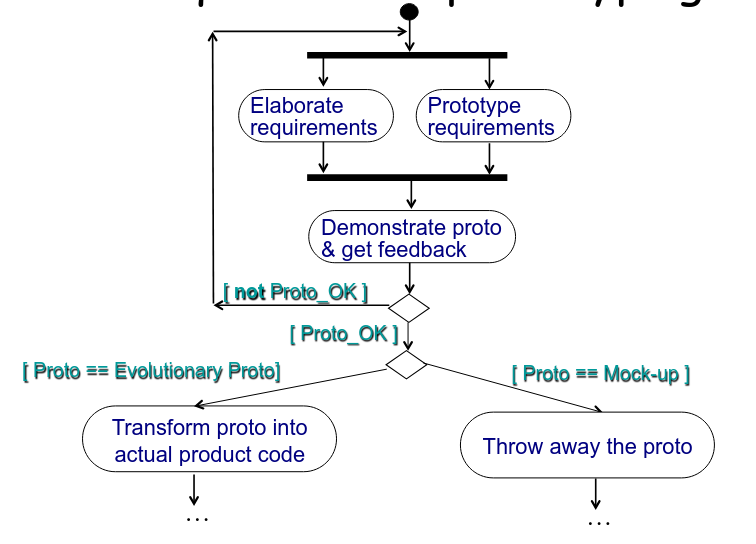
\includegraphics[width=0.7\textwidth]{pictures/schemaPrototipo.png}
	\caption{Schema di sviluppo di un prototipo}
\end{figure}
Come per le altre tecniche di elicitazione, anche i prototipi presentano vantaggi e svantaggi:
\begin{itemize}
	\item \textbf{Pro}
	\begin{itemize}
		\item Assaggio concreto di come sarà il software, vengono quindi chiariti i requisiti, elicitati quelli nascosti, in generale si miglioano quelli raccolti.
	\end{itemize}
	\item \textbf{Contro}
	\begin{itemize}
		\item Possono essere fuorvianti, alzando troppo le aspettative.
		\item Il codice prodotto di fretta senza cura può essere difficile da riutilizzare. 
		\end{itemize}
\end{itemize}
\subsection{Riutilizzo della conoscenza}
Come obiettivo vogliamo velocizzare il processo di elicitazione riutilizzando la conoscenza acquisita in progetti pregressi affini.
In generale il processo consiste in:
\begin{enumerate}
	\item Ottenere la conoscenza rilevante proveniente da altri sistemi.
	\item Trasportarla nel sistema target.
	\item Validare il risultato, adattarlo se necessario e integrarlo con la conoscenza già conseguita. 
\end{enumerate}
La conoscenza potrebbe dipende o meno dal dominio. Chiaramente sono presenti vantaggi e svantaggi:
\begin{itemize}
	\item \textbf{Pro}
	\begin{itemize}
		\item Il processo avviene in maniera naturale.
		\item Una guida significative riduce lo sforzo necessario per l'elicitazione.
		\item Vengono ereditate strutture e qualità di aspetti astratti di dominio.
		\item Efficace per completare i requisiti con aspetti mancanti.
	\end{itemize}
	\item \textbf{Contro}
	\begin{itemize}
		\item Utile solo se il dominio astratto è sufficientemente simile e accurato.
		\item Definire domini astratti per facilitare il riuso è difficile.
		\item Richiede lavoro per valutare l'integrazione.
		\item Affinità parziali richiedono adattamenti insidiosi.
	\end{itemize}
\end{itemize}
\subsection{Modelli minori}
\begin{itemize}
	\item \textbf{Card sorting:} chiedere agli stakeholder di partizionare un insieme  di cartelli
	\begin{itemize}
		\item Ogni carta cattura un concetto testualmente o graficamente.
		\item Le carte vengono raggruppate secondo criteri dello stakeholder.
		\item L'obiettivo consiste nell'acquisire ulteriori informazioni riguardanti concetti che sono già stati elicitati.
		\item Per ogni sottoinsieme di carte viene chiesto le proprietà comuni implicite utilizzate per raggrupparle.
		\item Iterare con le stesse carte per nuovi raggruppamenti e proprietà. 
	\end{itemize}
\end{itemize}
\begin{itemize}
	\item \textbf{Data collection:} dati marketing, statistiche d'utilizzo, metriche di performance, costi\dots
	\begin{itemize}
		\item L'obiettivo è raccogliere fatti e cifre non documentati. Ciò viene fatto tramite esperimenti o una selezione di dataset di rappresentativi presi da fonti disponibili.
		\item Potrebbe complementare lo studio di background. 
	\end{itemize}
\end{itemize}
\section{Tecniche di elicitazione stakeholder-driven}
\subsection{Interviste}
Tecnica primaria per elicitare la conoscenza.
\begin{enumerate}
	\item Selezionare lo stakeholder specificatamente per l'informazione da acquisire.
	\item Organizzare un incontro con l'intervistato, fare domande e segnare le risposte.
	\item Scrivere un report con trascritto dell'intervista.
	\item Sottomettere il report per la validazione e il rifinimento.
\end{enumerate}
Un'intervista può coinvolgere più stakeholder, ciò può far risparmiare tempo ma può anche inibire la comunicazione.
Le interviste possono essere di due tipi:
\begin{itemize}
	\item \textbf{Strutturate:} domande predefinite, specifiche per la ragione dell'intervista. Alcune domande aperte, altre a risposta multipla. 
	\item \textbf{Non strutturate:} nessuna domanda predefinita, discussione libera sul sistema as-is, problemi percepiti, soluzioni proposte. Vengono esplorati problemi che potrebbero essere stati tralasciati.
\end{itemize}
Una intervista efficace dovrebbe mischiare le due modalità, partendo da una parte strutturata per poi aprirsi a domande più libere quando necessario.
È preferibile seguire le seguenti linee guida:
\begin{itemize}
    \item Preparati in anticipo, concentrandoti sul problema giusto al momento giusto
    \begin{itemize}
        \item Evita domande ovvie per l’intervistato (es. studia prima il suo background)
        \item Progetta in anticipo una sequenza di domande specifica per quell’intervistato
    \end{itemize}

    \item Centra l’intervista sul lavoro e sulle preoccupazioni dell’intervistato
    \item Mantieni il controllo dell’intervista
    \item Fai sentire l’intervistato a proprio agio
    \begin{itemize}
        \item All’inizio: rompi il ghiaccio, fornisci una motivazione, poni domande semplici
        \item Considera la persona, non solo il suo ruolo
        \item Mostrati sempre come un partner affidabile
        \item Fai domande del tipo ``Perché?''
    \end{itemize}

    \item Evita certi tipi di domande:
    \begin{itemize}
        \item di parte o faziose
        \item affermative
        \item ovvie o impossibili da rispondere per quell’intervistato
    \end{itemize}

    \item Rivedi e struttura le trascrizioni dell’intervista finché sono ancora fresche nella mente
    \begin{itemize}
        \item includendo reazioni personali, atteggiamenti, ecc.
    \end{itemize}

    \item Mantieni l’intervistato coinvolto
    \begin{itemize}
        \item co-rivedi la trascrizione per validazione e perfezionamento
    \end{itemize}
\end{itemize}
\subsection{Osservazioni e studi etnografici}
A volte comprendere un'azione è più facile osservandola piuttosto che tramite una spiegazione verbale o testuale.
L'osservazione può essere fatta in due modi:
\begin{itemize}
	\item \textbf{Passiva:} nessuna interferenza con colui che esegue l'azione.
	\begin{itemize}
		\item Osservazione dall'esterno, registrazione, trascritti e analisi.
		\item Analisi di protocollo: gli esecutori spiegano cosa fanno mentre lo fanno.
		\item Studio etnografico: osservazione prolungata per comprendere proprietà emergenti del gruppo sociale coinvolto.
	\end{itemize}
	\item \textbf{Attiva:} l'osservatore partecipa all'azione, diventando anche un membro del gruppo.
\end{itemize}

\end{document}